\chapter{Analysis}

The objective of this analysis is to validate the model and the simulation. The required torque calculated in the maths model and simulated in Drake is compared with the experimental data to determine the validity of the maths model and the simulation.

\section{Quantitative comparison}

The torque measurement experiment gives two values for each stage of motion, the torque required to cause some partial movement, and the torque required to cause full movement. These values will be referred to as $T_{Partial}$ and $T_{Full}$ respectively, and are shown in Figure \ref{fig:torque-experiment}.\\

\begin{figure}[!h]
	\centering
	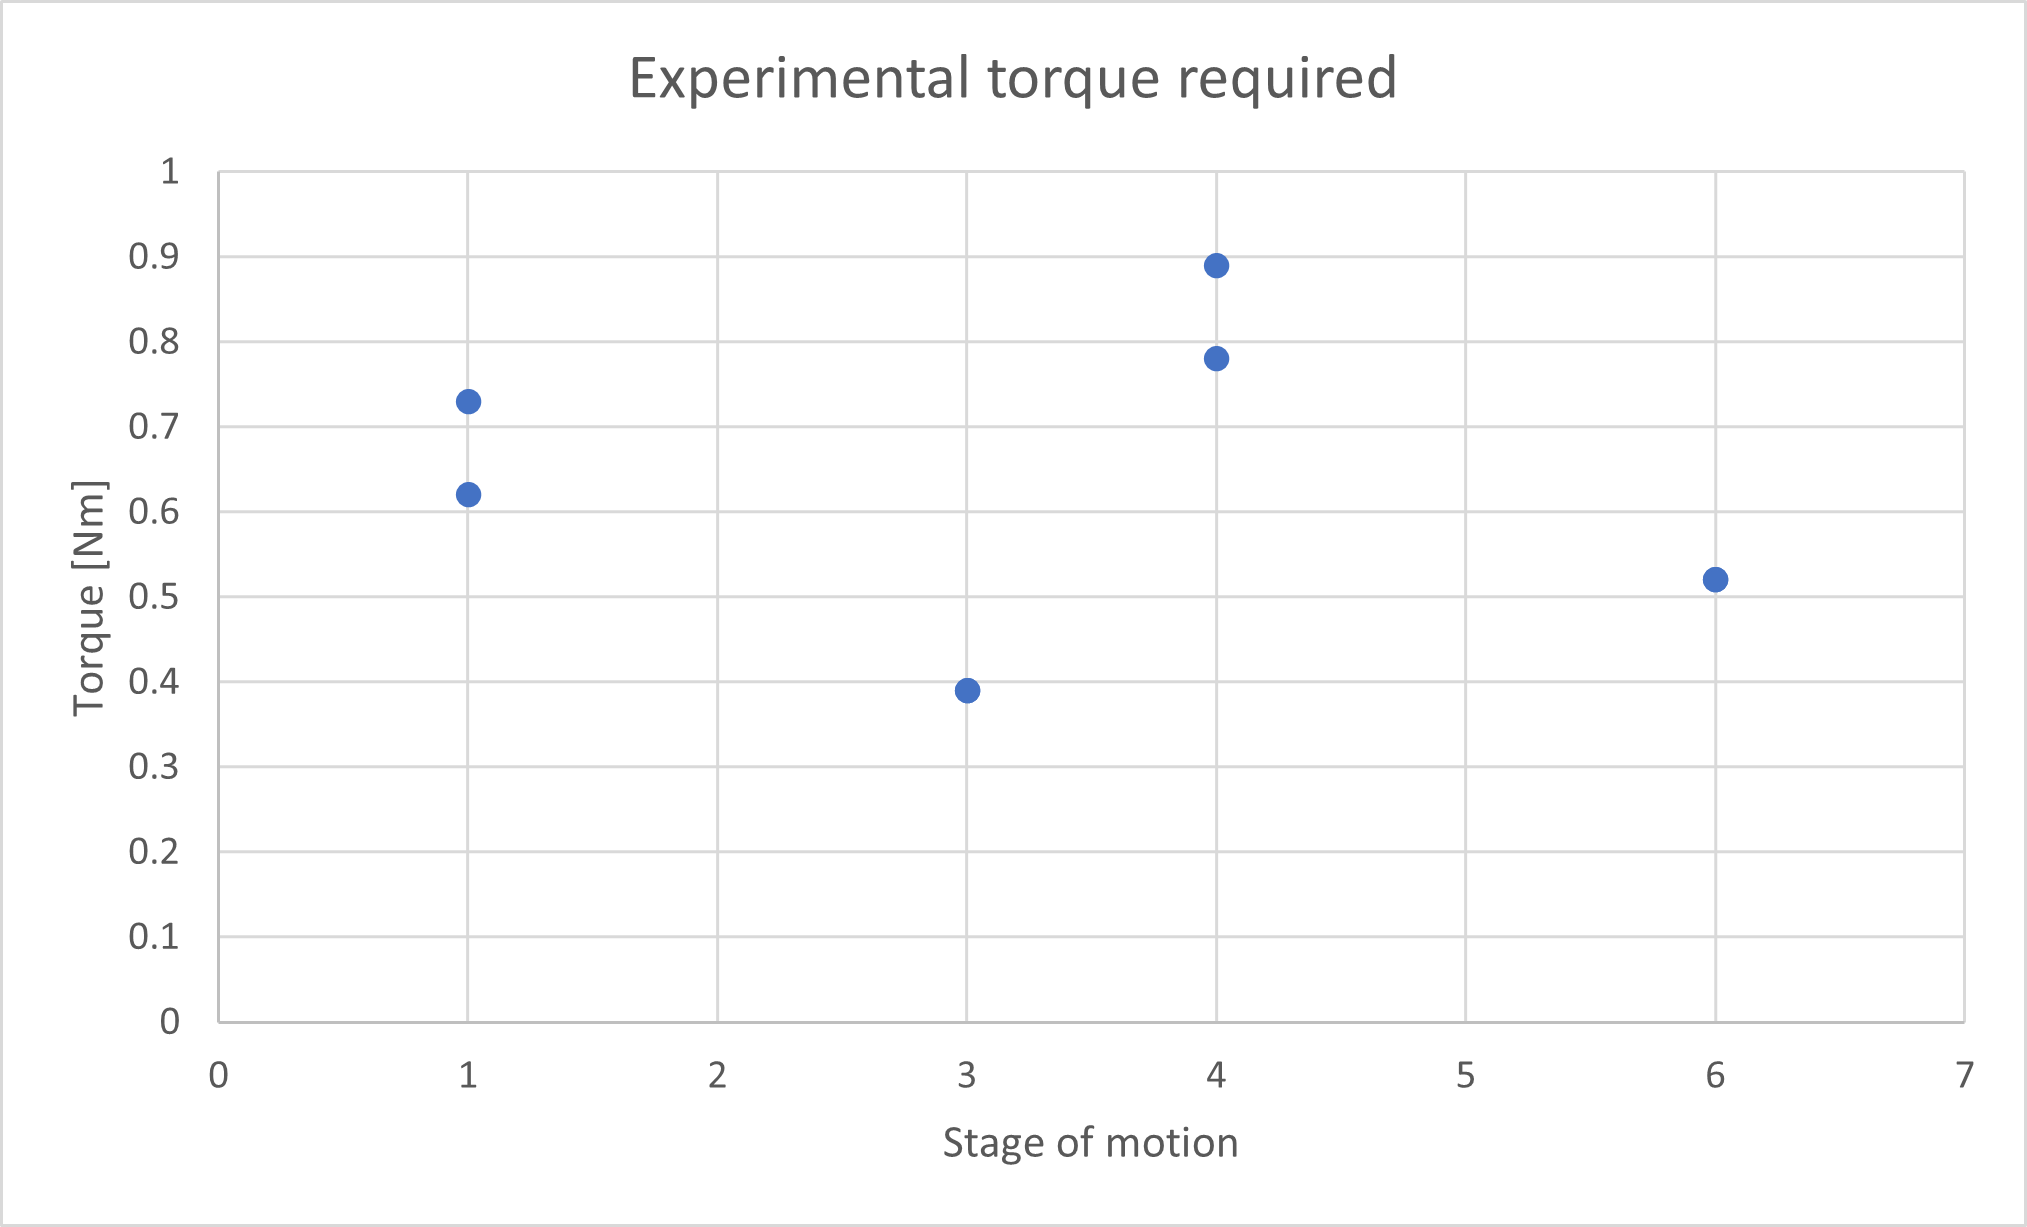
\includegraphics[width=0.8\textwidth]{plots/torque-experiment-forecasted}
	\caption{Required torques for each stage determined experimentally}
	\label{fig:torque-experiment}
\end{figure}

In Figure \ref{fig:torque-experiment}, there are two points for each stage, the higher of which is $T_{Full}$ and the lower is $T_{Partial}$. In cases where only a single point is present, there was no torque that would cause a partial movement; meaning that if the torque is high enough to start the movement, it is also high enough to complete the movement. Stages 0, 2, and 5 are omitted as the device does not push against gravity in these stages, so the torque required is negligible.\\

To determine the required torque in the simulation, the torque measurement experiment is simulated. The torque required across each stage of motion has already been calculated using the maths model, as shown in Figure \ref{fig:bigplot}. The required torque at the start of each stage is equivalent to $T_{Partial}$, as this is the torque that will cause the motion to start. The highest required torque for each stage is $T_{Full}$, as if the device can output this torque it will be able to complete the full stage of motion. The required torque produced by the simulation and the maths model are shown side by side with the experimental data in Figure \ref{fig:torque-comparison}.\\

\begin{figure}[!h]
	\centering
	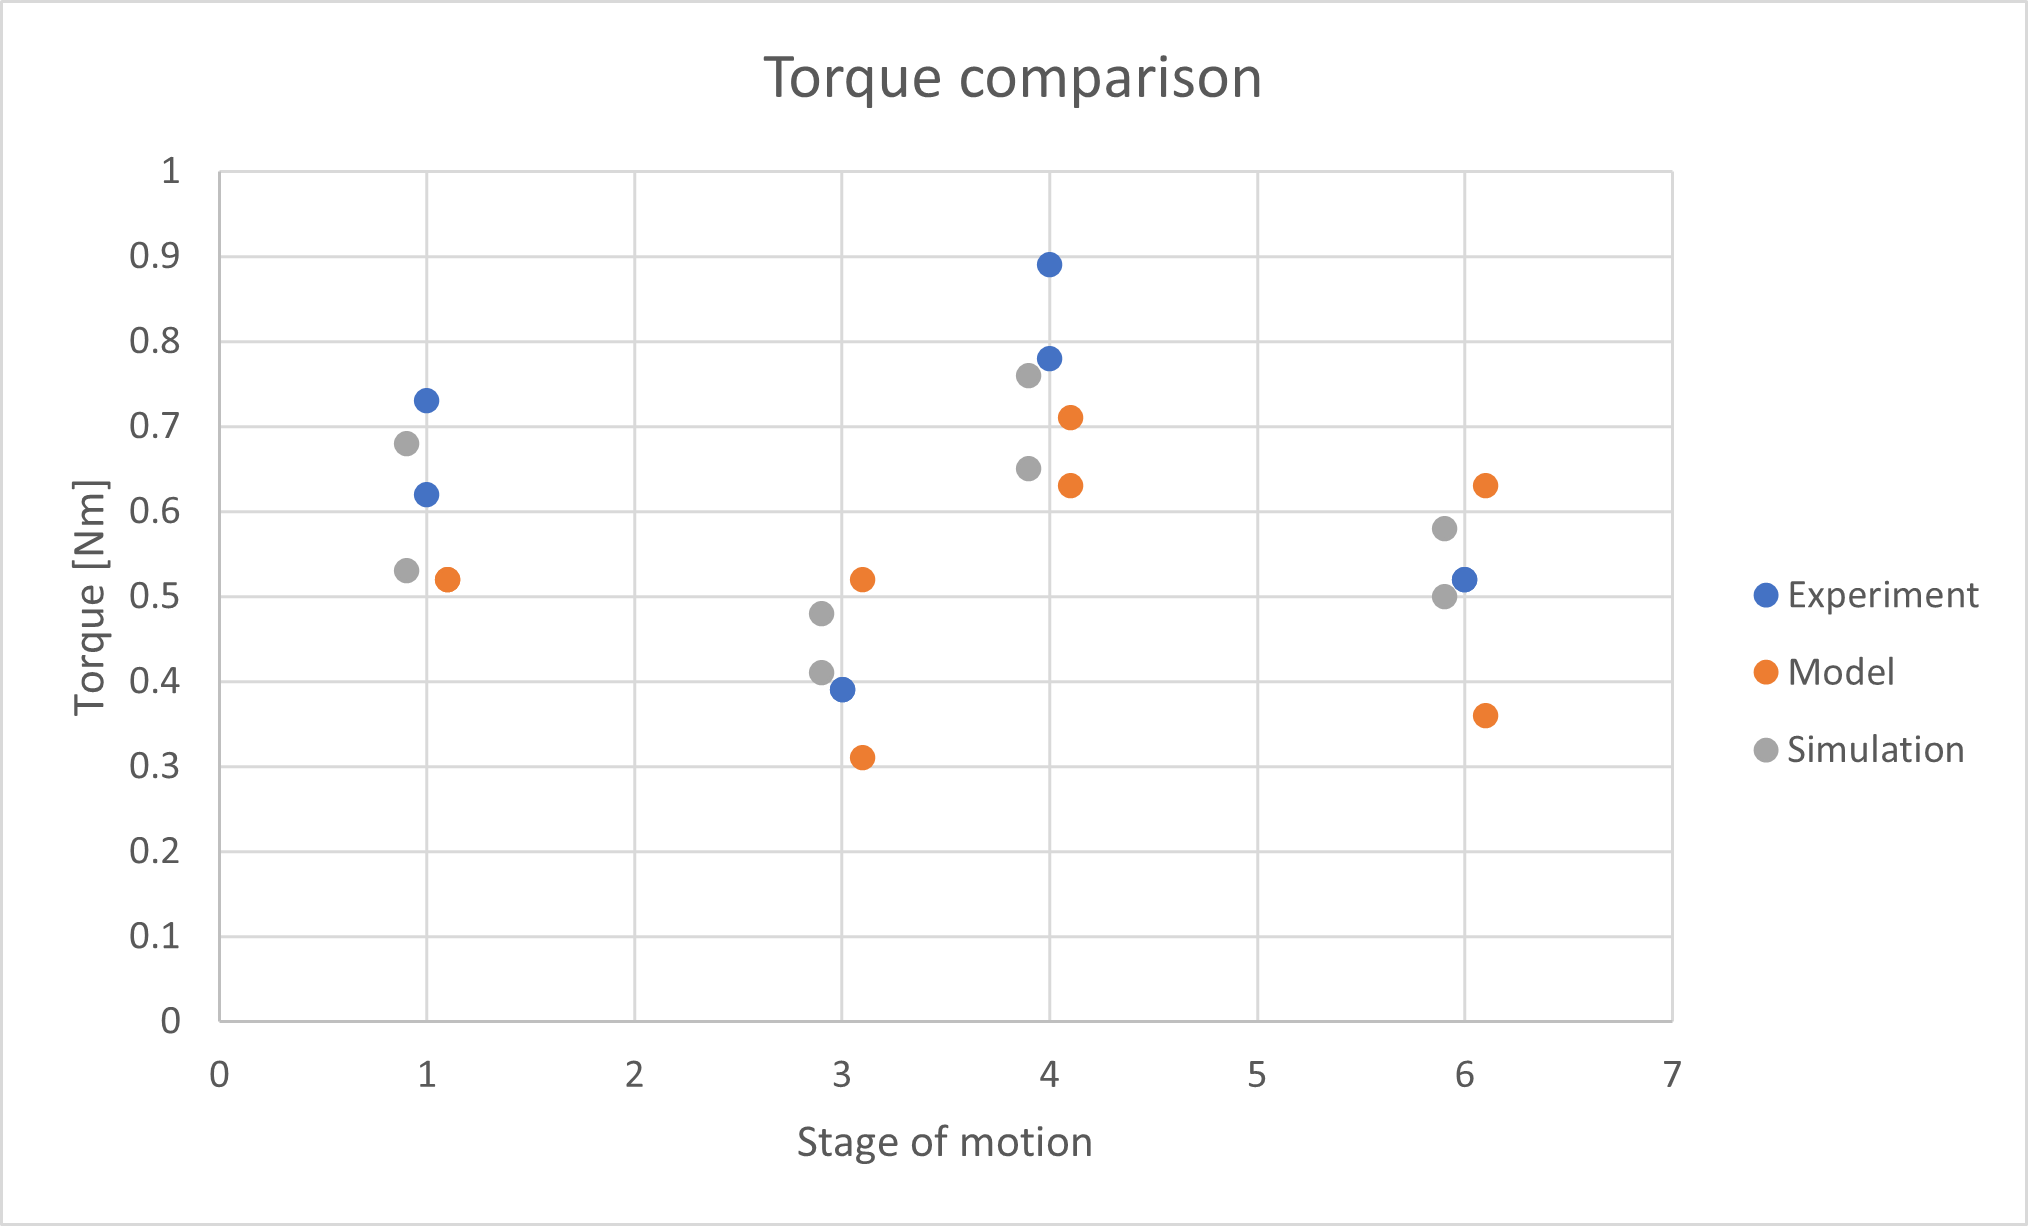
\includegraphics[width=0.8\textwidth]{plots/torque-comparison-forecasted}
	\caption{Required torques for each stage from different sources.}
	\label{fig:torque-comparison}
\end{figure}

Figure \ref{fig:torque-comparison} shows that the model, simulation, and experiment all produce similar values. In Stages 1 and 4, the model and simulation both produce a lower required torque than the device actually needs. In Stages 3 and 6, the device needs less torque to complete the motion than the model and simulation predict.\\
To test the accuracy of the model and simulation across a range of design parameters, the experiment and comparison were repeated twice, once with a 60 cm long tail in place of the 30 cm one, and once with a 340 g mass attached to the body of the device. The comparison between these results are shown in Figures ??? and ???.  
\\
 
\section{Assessment of error}

Table \ref{tab:error} shows the percentage error of the required torque produced by the model and simulation. The simulation is shown to be more accurate than the maths model at every data point, and the point with the highest error for both is the torque required to cause complete motion in Stage 3.\\
 

\begin{table}[!ht]
	\centering
	\caption{Percentage error of required torque for each stage of motion in the model and simulation.}
	\label{tab:error}
	\begin{tabular}{|l|l|l|l|l|l|l|l|l|}
		\hline
		~ & Stage 1 & ~ & Stage 3 & ~ & Stage 4 & ~ & Stage 6 & ~ \\ \hline
		~ & Partial & Full & Partial & Full & Partial & Full & Partial & Full \\ \hline
		Model & -16.1\% & -28.8\% & -20.5\% & 33.3\% & -19.2\% & -20.2\% & -30.8\% & 21.2\% \\ \hline
		Simulation & -14.5\% & -6.8\% & 5.1\% & 23.1\% & -16.7\% & -14.6\% & -3.8\% & 11.5\% \\ \hline
	\end{tabular}
\end{table}

Identifying the source of the error is not essential for the purposes of informing design, one can simply design the motors to have at least 1.5 times the calculated required torque. However, analysing the source of this error is important in order to improve future versions of the model.\\

In Stage 1, the model predicts that there is no torque that will cause partial movement. As the device lifts the torque required decreases, so if the torque is high enough to start lifting, it is high enough to complete Stage 1 motion. However, Figure \ref{fig:torque-comparison} shows that there is a range of torques that produce partial motion in the experimental and simulated data. The most likely cause for this is that some assumption made in the maths model is invalid. Although the calculations are done differently, the simulation is subject to the same rigid body and friction assumptions as the maths model. The main discrepancy between the two is that the simulation allows motion in three dimensions while the model is limited to two. As there is a large difference between the results of the model and the simulation, it is likely that the three-dimensional movement is what allows the device to get stuck part way during Stage 1. Initial tests showed that if one of the LIMs moves ahead of the other, the device will tip slightly, putting more weight on the LIM that falls behind, preventing the LIM from lifting unless it has excessive torque. An example of this is shown in Figure ???. It is likely that even when the LIMs appear to move in unison, even a slight imbalance can cause the motion to stop part way when the motor torque is close to the required torque. To address this error, one could update the maths model to allow movement in three dimensions, however this would drastically increase the complexity and the calculation time of the model, and is excessive when tools for three-dimensional simulation such as Drake are readily available.\\

In Stages 3 and 6, the experiment shows that there is no torque that causes partial motion. However, the simulation indicates that there is a small range of torques that cause partial motion, and the maths model indicates that there is a large range of torques that cause partial motion. Both the simulation and the maths model also indicate that the required torque is higher than the experimental value. The reason for this error in the maths model is because it incorrectly assumes that the frame of the LIM will not come into contact with the step. When the device climbs in Stages 3 and 6, the frame of the LIM slides along the edge of the step while the front wheel pulls the device up the step, which is illustrated in Figure ???. The step supports the frame of the LIM, so that the device needs less torque in order to overcome gravity, which explains why the actual device needs less torque to complete the stage of motion than the model predicted. To address this error, the model could be updated to model the contact between the step and the LIM frame, however this would be difficult to do analytically as the LIM frame has an irregular shape. The simulation does model the contact between the LIM frame and the step, however it still indicates that there should be partial movement and that the required torque is higher than the experimental value. This is likely because the coefficient of friction between the LIM frame and the step is higher in the simulation than in reality. Coefficients of friction in Drake default to 1.0, which is much larger than most real surfaces will have. This error could be eliminated by setting the coefficient of friction of the LIM frame to a lower value. \\

Another potential source of error comes from the calibration of the motors. The voltage torque calibration experiment in Section \ref{sec:Voltage-torque calibration} was used to produce Equation \ref{eqTorqueVoltage}, which was later used to calculate the experimental required torque from the measured voltage. An error in the calibration method could cause all of the experimental results to be off by a constant factor. The method of this experiment involved using the motors to lift a weight with a lever. Typically in this style of experiment, the motor torque would reach an equilibrium with the moment from the weight and the lever would stop moving. However, as the gearbox on the motors is self-locking, the lever cannot move in reverse. This means that if the lever ever lifts beyond the equilibrium point, it will not fall back to the equilibrium point and the recorded lever angle will be higher than the motors could actually output. There are two possible ways that the lever can lift beyond the equilibrium point in this experiment. Firstly, if the lever and the mass have a significant momentum when they reach the equilibrium point, they will move beyond it; this is mitigated by the high gear ratio on the motor which causes it to move quite slowly. Secondly, as the mass is attached to the lever by string, it can act as a pendulum. The swing of the pendulum will sometimes make it easier for the lever to lift, and sometimes make it harder. This combines with the self-locking gearbox to cause the lever to inch forward while the pendulum is helping it, then the gearbox locks when the pendulum swings the other way. This is visualised in Figure ???. The net result is that the lever moves slightly beyond the equilibrium point. \\
If the motors incorrectly calibrated and appear to produce more torque than they actually do, it would help explain why the experimental torques are higher than the modelled and simulated torques in Stages 1 and 3. This error could be mitigated by attaching the mass directly to the lever rather than by string.

